\documentclass[aspectratio=169]{beamer}


\usepackage[utf8]{inputenc}
\usepackage[T1]{fontenc}
\usepackage{lmodern}

\usepackage{hyperref}
\hypersetup{
    colorlinks=true,
    linkcolor=black
}

\usepackage{amsmath}
\usepackage{amssymb}
\usepackage{amsfonts}
\usepackage{bm}

\usepackage{listings}
\usepackage{minted}
\lstset{basicstyle=\ttfamily}

\usepackage{algorithm,algorithmicx,algpseudocode}

\usepackage{xspace}

\usepackage[]{todonotes}

\usepackage{beamerthemeuclcryptov2}

\AtBeginSection[]
{
    \begin{frame}<beamer>
        \frametitle{Content}
        \tableofcontents[currentsection]
    \end{frame}
}

\DeclareMathOperator*{\expectation}{\mathbb{E}}
\DeclareMathOperator*{\variance}{\mathbb{V}}
\DeclareMathOperator*{\argmax}{\arg\max}


\title{Side-channel cryptanalysis of a masked AES with SCALib}

\author[G. Cassiers]{
    Gaëtan Cassiers
}

\begin{document}

\begin{frame}{}
    \maketitle
    \begin{columns}
        \begin{column}{0.15\textwidth}
            \includegraphics[width=\textwidth]{logos/uclouvain.png}
        \end{column}
        \begin{column}{0.08\textwidth}
            \includegraphics[width=\textwidth]{logos/crypto_group.jpg}
            % TODO logo simple-crypto
        \end{column}
    \end{columns}
    \vspace*{3ex}
    \begin{center}
        Download the dataset:~\url{https://tinyurl.com/ascad-5k} (1.3~GB) \\
        % TODO https://drive.google.com/file/d/12_vaKztMGigkKn3YmOKqLj4E1d6ItdaQ/view?usp=sharing
        Slides available at~\url{https://github.com/simple-crypto/scalib-tutorial}
    \end{center}
    \vspace*{2ex}
\end{frame}

%\begin{frame}{Acknowledgements}
%    \begin{itemize}
%        \item Olivier Bronchain
%        \item SCALib contributors
%    \end{itemize}
%\end{frame}

\begin{frame}{Table of Contents}
    \tableofcontents
\end{frame}

\section{Introduction}

\begin{frame}{Attack context}
    \begin{center}
        \emph{How secure is my implementation?}
    \end{center}

    Worst-case attack:
    \begin{itemize}
        \item Assume all implementation details are known.
        \item Powerful profiling available (including knowledge of the masks).
        \item Profile \& attack on the same device.
    \end{itemize}
\end{frame}

\begin{frame}{SCALib: A Side-Channel Analysis Library}
    \begin{itemize}
        \item Flexible \& Simple: a Python library working on numpy arrays.
        \item High performance: expensive computations are optimized with native code and multi-threaded.
        \item Scalability thanks to streaming APIs.
    \end{itemize}
    \begin{center}
        See docs at \url{https://scalib.readthedocs.io/}.
    \end{center}
\end{frame}

\begin{frame}{ASCAD: ANSSI's Side-Channel Analysis Dataset}
    ASCADv1 variable key:
    \begin{itemize}
        \item Released in 2018.
        \item 300k traces, 250k points in full traces.
        \item 8-bit smart card.
        \item Often used in (deep learning) SCA research.
    \end{itemize}
\end{frame}

\begin{frame}{A table-based masked AES implementation}
    \begin{algorithmic}
        \ttfamily
        \State Input: masked key bytes $(k^{(0)}_0, k^{(0)}_1),\dots, (k^{(15)}_0, k^{(15)}_1)$.
        \State Input: masked plaintext bytes $(p^{(0)}_0, p^{(0)}_1),\dots, (p^{(15)}_0, p^{(15)}_1)$.
        \State Input: randomness bytes $r_{in}$, $r_{out}$, masked sbox table $MskSbox$.
        \State // Add round key
        \For{$i=0,\dots,15$}
            \State $x^{(i)}_0 \gets k^{(i)}_0 \oplus p^{(i)}_0$
            \State $x^{(i)}_1 \gets k^{(i)}_1 \oplus p^{(i)}_1$
            \State $x^{(i)}_{rin} \gets (x^{(i)}_0 \oplus r_{in}) \oplus x^{(i)}_1$
            \State $x^{(i)}_{rout} \gets MskSbox(x^{(i)}_{rin})$
            \State $y^{(i)}_0 \xleftarrow{\$} \mathbb{F}_{256}$
            \State $y^{(i)}_1 \gets (x^{(i)}_{rout} \oplus y^{(i)}_0) \oplus r_{out}$.
        \EndFor
        \State // ...
    \end{algorithmic}
\end{frame}

\begin{frame}{A simple attack on ASCAD}
    \begin{center}
        \emph{Profile all intermediate variables in the computation, recombine these to get the key.}
    \end{center}
    \pause

    \begin{enumerate}[<+->]
        \item Selection of Points Of Interest (POIs) for each intermediate
            \begin{itemize}[<.->]
                \item To reduce leakage's dimensionality.
                \item Select $k$ points with highest Signal-to-Noise Ratio (SNR).
            \end{itemize}
        \item Build templates with Linear Discriminant Analysis (LDA)
            \begin{itemize}[<.->]
                \item Gaussian Templates with pooled covariance matrix \& dimensionality reduction.
                \item Outputs probability distribution (over $\mathbb{F}_{256}$) for each intermediate.
            \end{itemize}
        \item Recombine intermediates with Soft-Analytical Side-Channel Attack (SASCA)
            \begin{itemize}[<.->]
                \item Bayesian inference: find key distribution given intermediate's distributions.
                \item (Approximate) solution: (loopy) belief propagation.
            \end{itemize}
        \item Evaluate the attack: find the key rank
            \begin{itemize}
                \item Also known as Guessing Entropy (GE).
            \end{itemize}
        \item (Bonus) Leakage assessment with uni- and bi-variate T-test
    \end{enumerate}

    \uncover<8->{\textit{Attack introduced in} \url{https://eprint.iacr.org/2021/817}}
\end{frame}

\section{Getting Started}
\begin{frame}{Setup}
    Follow instructions in the notebook:
    \begin{center}
        \url{https://github.com/simple-crypto/scalib-tutorial/blob/main/Tutorial.ipynb}
    \end{center}

    You may run the code on your laptop (recommended) or use a Google Colab notebook.

    % TODO: local download link for data.
\end{frame}


\begin{frame}{Step 0: Plot a trace}
    Result:
    \begin{center}
        \includegraphics[width=\textwidth]{figures/res_step0.png}
    \end{center}
\end{frame}

\section{Attack Implementation}
\begin{frame}{Step 1: SNR + POI}
    For every variable $v$ among $r_{in}, r_{out}, x^{(i)}_0, x^{(i)}_1, y^{(i)}_0, y^{(i)}_1$,
    \begin{enumerate}
        \item Compute the SNR for each point $k$ in the trace:
            \[
                \textsf{SNR}_{v,k} = \frac{
                    \variance_{v}\left(\expectation_{l_k}(l_k)\right)
                }{
                    \expectation_{v}\left(\variance_{l_k}(l_k)\right)
                }
            \]
        \item Select the $N_{\textsf{POIs}}=512$ points with higest SNR for each variable:
            \[
                \textsf{POIs}_{v} = \argmax_k \textsf{SNR}_{v,k}
            \]
    \end{enumerate}

    Useful classes/functions:
    \href{https://scalib.readthedocs.io/en/stable/source/api/scalib.metrics.SNR.html}{scalib.metrics.SNR},
    \href{https://numpy.org/doc/stable/reference/generated/numpy.argsort.html}{numpy.argsort}

    \bigskip

    Trick: \texttt{right clik > New Console for Notebook}
\end{frame}
\begin{frame}{Step 1: result}
    \begin{center}
        \includegraphics[width=\textwidth]{figures/res_step1.png}
    \end{center}
\end{frame}

\begin{frame}[containsverbatim]{Step 1: Solution}

Compute the SNR with:
\begin{minted}{python}
for v in tqdm(variables, desc="SNR Variables"):
    snr = SNR(nc=256)
    x = labels[v].reshape((settings.profile, 1))
    snr.fit_u(traces, x)
    snrs[v] = snr.get_snr()[0, :]
\end{minted}

Recover the POIs with:
\begin{minted}{python}
for v, snr in snrs.items():
    poi = np.argsort(snr)[-settings.poi :].astype(np.uint32)
\end{minted}
\end{frame}

\begin{frame}{Step 2: LDA}
    For every variable $v$:
    \begin{enumerate}
        \item compute a linear discriminant analysis model based on the POIs,
        \item make a scatter plot of the 2D-projected features,
        \item predict a probability distribution of the variable for a new trace.
    \end{enumerate}

    The LDA model is both
    \begin{itemize}
        \item a linear dimensionality reduction tool (that maximizes SNR in projected dimensions),
        \item a Bayesian classification tool (a.k.a. pooled Gaussian templates).
    \end{itemize}

    Useful classes/functions:
    \href{https://scalib.readthedocs.io/en/stable/source/api/scalib.modeling.LDAClassifier.html}{scalib.modeling.LDAClassifier}
\end{frame}

\begin{frame}{Step 2: result}
    \begin{center}
        \includegraphics[width=.6\textwidth]{figures/res_step2.png}
    \end{center}
\end{frame}


\begin{frame}[containsverbatim]{Step 2: Solution}

Compute the LDA with:
\begin{minted}{python}
for v in tqdm(variables, desc="LDA Variables"):
    lda = scalib.modeling.LDAClassifier(nc=256, p=settings.dim)
    lda.fit_u(traces[:, pois[v]], labels[v])
    lda.solve()
\end{minted}

\end{frame}

\begin{frame}{Step 3: SASCA}
    \begin{columns}
        \begin{column}{0.4\textwidth}
            \begin{enumerate}
                \item Implement factor graph
                \item Add evidence from LDA
                \item Run belief propagation
                    \begin{itemize}
                        \item Remark: no cycle!
                    \end{itemize}
            \end{enumerate}
        \end{column}
        \begin{column}{0.5\textwidth}
            \resizebox{\textwidth}{!}{
                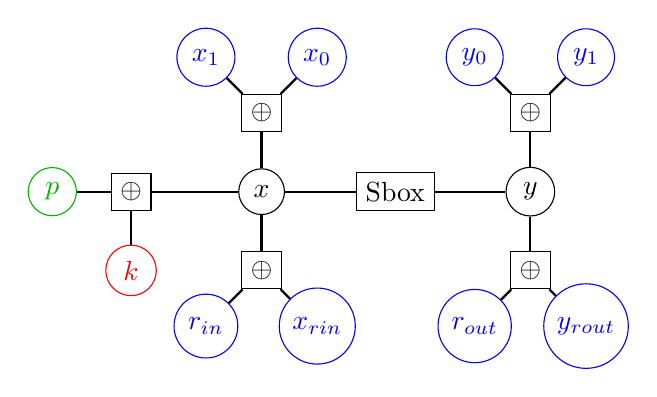
\begin{tikzpicture}
                    \node[draw,rectangle](xor1) {$\oplus$};
\node[color=blue,draw,circle,above right of=xor1] (x0) {$x_0$};
\node[color=blue,draw,circle,above left of=xor1] (x1) {$x_1$};
\node[draw,circle,below of=xor1](x){$x$};
\node[draw,rectangle,below of=x](xor2) {$\oplus$};
\node[color=blue,draw,circle,below left of=xor2](rin) {$r_{in}$};
\node[color=blue,draw,circle,below right of=xor2](xrin) {$x_{rin}$};


\node[rectangle,draw,right =.9cm of x] (sbox) {Sbox};
\node[circle,draw,right =.9cm of sbox] (y) {$y$};
\node[rectangle,draw,below of=y] (xor3) {$\oplus$};
\node[circle,color=blue,draw,below left of=xor3] (rout) {$r_{out}$};
\node[circle,color=blue,draw,below right of=xor3] (yrout) {$y_{rout}$};

\node[draw,rectangle,above of=y](xor4) {$\oplus$};
\node[color=blue,draw,circle,above left of=xor4](y0) {$y_0$};
\node[color=blue,draw,circle,above right of=xor4](y1) {$y_1$};



\node[rectangle,draw,left =1.1cm of x] (xorp) {$\oplus$};
\node[color=green!70!black,circle,draw,left of=xorp](p){$p$};
\node[color=red,circle,draw,below of=xorp](k){$k$};

\draw[thick] (p) -- (xorp) -- (x);
\draw[thick] (k) -- (xorp);

\draw[thick] (x0) -- (xor1) -- (x1);
\draw[thick] (xor1) -- (x) -- (sbox);
\draw[thick] (rin) -- (xor2) -- (xrin);
\draw[thick] (x) -- (xor2);

\draw[thick] (y0) -- (xor4) -- (y1);
\draw[thick] (xor4) -- (y) -- (sbox);
\draw[thick] (rout) -- (xor3) -- (yrout);
\draw[thick] (y) -- (xor3);

                \end{tikzpicture}
            }
        \end{column}
    \end{columns}

    Useful classes/functions:
    \href{https://scalib.readthedocs.io/en/stable/source/api/scalib.attacks.FactorGraph.html}{scalib.attacks.FactorGraph}.
\end{frame}
\begin{frame}{Step 3: result}
    \begin{center}
        \includegraphics[width=\textwidth]{figures/res_step3.png}
    \end{center}
\end{frame}
\begin{frame}[containsverbatim]{Step 3: solution}
    \small
For each of the bytes, run:
\begin{minted}{python}
# Init the sasca with the factor graph for a single trace
graph = scalib.attacks.FactorGraph(sasca_graph, {"sbox": SBOX})
# Set the labels for the plaintext byte
bp = scalib.attacks.BPState(graph, 1, {"p": labels[f"p_{i}"].astype(np.uint32)})
# Set the initial distri. for target var. 'vs' if it is in the graph
for v in target_variables(i):
    vs = v.split('_')[0]
    if vs in graph.vars():
        # Assign the distribution of vs
        prs = ldas[v].predict_proba(traces[:, pois[v]])
        bp.set_evidence(vs, prs)
# Run 3 iterations of belief propagation
bp.bp_loopy(it=3, initialize_states=True)
byte_distribution = bp.get_distribution(f"k")
\end{minted}
\end{frame}

\begin{frame}{Step 4: Key rank estimation}
    Key rank (a.k.a. Guessing Entropy):
    \[
        r = \left\vert\left\{
            k \in \mathcal{K} \;|\; \tilde{\Pr}[K=k] \ge \tilde{\Pr}[K=k*]
            \right\}\right\vert
    \]
    where $k*$ is the correct key.

    Easy to compute on single byte, harder for large keys.

    \begin{enumerate}
        \item Compute the rank for each of the key bytes.
        \item Compute an estimation of the rank of the full key.
    \end{enumerate}

    Useful classes/functions:
    \href{https://numpy.org/doc/stable/reference/generated/numpy.count_nonzero.html}{numpy.count\_nonzero},
    \href{https://scalib.readthedocs.io/en/stable/source/api/scalib.postprocessing.rankestimation.html}{scalib.postprocessing.rankestimation}.
\end{frame}
\begin{frame}{Step 4: result}
    \begin{center}
        \includegraphics[width=\textwidth]{figures/res_step4.png}
    \end{center}
\end{frame}

\begin{frame}[containsverbatim]{Step 4: solution}
\begin{minted}{python}
def eval_rank(secret_key, key_distribution):
    """Returns the rank of the true key"""

    # Floor the key_distribution to avoid numerical issues
    key_distribution[np.where(key_distribution < 1e-100)] = 1e-100

    # Compute the rank of the
    log2distribution = np.log2(key_distribution)
    rmin, r, rmax = scalib.postprocessing.rank_accuracy(
        -log2distribution, secret_key, max_nb_bin=2**20
    )

    return r

\end{minted}
\end{frame}

\begin{frame}{Step 5: Improved SASCA}
    Improve the attack by using the Sbox output (see right-hand part of the
    factor graph in Step~3).
\end{frame}

\begin{frame}{Step 5: result}
    \begin{center}
        \includegraphics[width=\textwidth]{figures/res_step5.png}
    \end{center}
\end{frame}

\begin{frame}[containsverbatim]{Step 5: solution}
    \footnotesize
    \begin{minted}{python}
SASCA_GRAPH_IMPROVED = """
    [... previous graph ...]

    VAR MULTI y
    VAR MULTI y0
    VAR MULTI y1
    VAR MULTI yrout
    VAR MULTI rout

    PROPERTY y = sbox[x]
    PROPERTY y = y0 ^ y1
    PROPERTY y = yrout ^ rout
"""
    \end{minted}
\end{frame}

\begin{frame}{Step 6: (Bonus) Leakage assessment}
    We run univariate (first and second-order) T-tests as well as a bivariate T-test.

    As classification bit, we cannot use the typical ``fix-vs-random'' with
    this dataset, we use a S-box input bit.
\end{frame}

\begin{frame}{Step 6: univariate result}
    \begin{center}
        \includegraphics[width=0.8\textwidth]{figures/res_step6a.png}
    \end{center}
\end{frame}

\begin{frame}{Step 6: bivariate result}
    \begin{center}
        \includegraphics[width=0.5\textwidth]{figures/res_step6b.png}
    \end{center}
\end{frame}

\begin{frame}[containsverbatim]{Step 6: solution}
    \footnotesize
    \begin{columns}
        \begin{column}{0.25\textwidth}
            \begin{center}
                Univariate
            \end{center}
    \begin{minted}{python}
ttest = Ttest(d=2)
ttest.fit_u(traces, x)
t = ttest.get_ttest()
    \end{minted}
        \end{column}
        \begin{column}{0.7\textwidth}
            \begin{center}
                Bivariate
            \end{center}
    \begin{minted}{python}
# Boolean matrix corresponding to the POI positions.
template = np.fromfunction(lambda i, j: i <= j, (n, n))
# Build POIS array from template
pois_idxs = np.nonzero(template)
pois_mat = np.vstack(pois_idxs).astype(np.uint32)
# Compute T-test
mttest = MTtest(d=2, pois=pois_mat)
mttest.fit_u(traces, x)
t = mttest.get_ttest()
    \end{minted}
        \end{column}
    \end{columns}
    % TODO bivariate solution ?
\end{frame}

\section{Conclusion}
\begin{frame}{A versatile attack}
    \begin{itemize}
        \item High robustness for hyperparameters (see \url{https://eprint.iacr.org/2021/817}).
        \item Similar to one of the winning attacks of the \href{https://ches.iacr.org/2023/challenge.php}{CHES~2023 challenge}.
        \item Similar flow works against post-quantum crypto \url{https://eprint.iacr.org/2023/1545}.
    \end{itemize}
\end{frame}

\begin{frame}{Other SCALib features}
    \begin{itemize}
        \item RLDA: a LDA that works with many classes (e.g. 16-bit or 32-bit states).
        \item Perceived information/Training information: evaluate quality of models.
    \end{itemize}

    See \url{https://scalib.readthedocs.io/en/stable/}

    Feature requests: \url{https://github.com/simple-crypto/SCALib/issues/new}
\end{frame}

\end{document}
